\documentclass{standalone}
\usepackage{tikz}
\usetikzlibrary{patterns, positioning}


\begin{document}
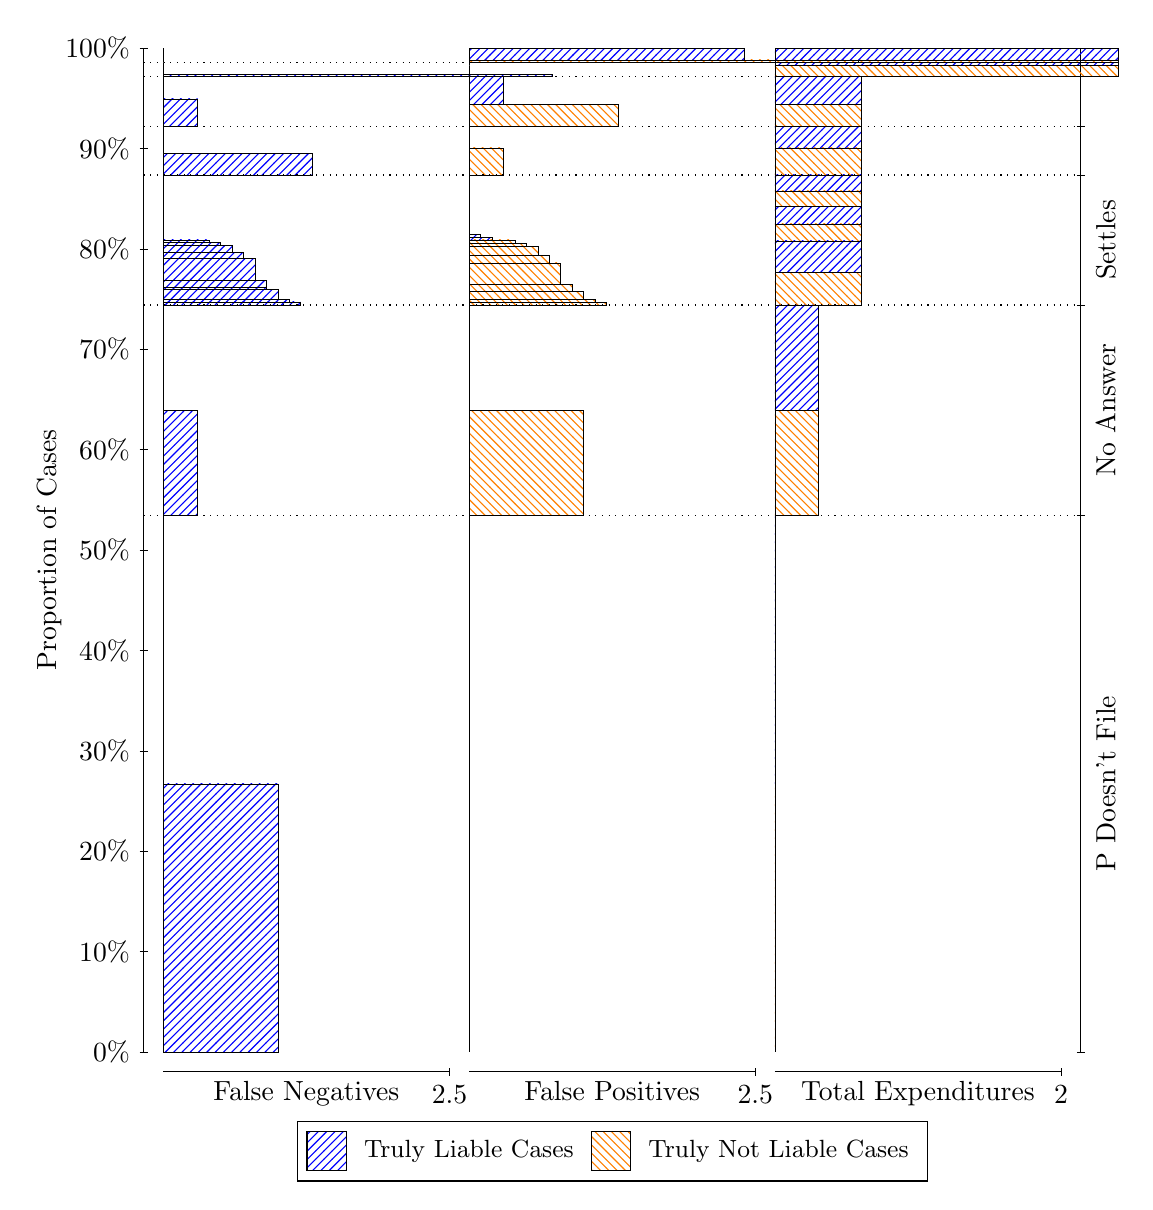
\begin{tikzpicture}
\draw[black, very thin] (1.5,1.75) -- (1.5,14.5);
\node[rotate=90, text=black, anchor=center] at (0.3, 8.125) {Proportion of Cases};
\draw[black, very thin] (1.45,1.75) -- (1.55,1.75);
\node[text=black, anchor=east] at (1.45, 1.75) {0\%};
\draw[black, very thin] (1.45,3.025) -- (1.55,3.025);
\node[text=black, anchor=east] at (1.45, 3.025) {10\%};
\draw[black, very thin] (1.45,4.3) -- (1.55,4.3);
\node[text=black, anchor=east] at (1.45, 4.3) {20\%};
\draw[black, very thin] (1.45,5.575) -- (1.55,5.575);
\node[text=black, anchor=east] at (1.45, 5.575) {30\%};
\draw[black, very thin] (1.45,6.85) -- (1.55,6.85);
\node[text=black, anchor=east] at (1.45, 6.85) {40\%};
\draw[black, very thin] (1.45,8.125) -- (1.55,8.125);
\node[text=black, anchor=east] at (1.45, 8.125) {50\%};
\draw[black, very thin] (1.45,9.4) -- (1.55,9.4);
\node[text=black, anchor=east] at (1.45, 9.4) {60\%};
\draw[black, very thin] (1.45,10.675) -- (1.55,10.675);
\node[text=black, anchor=east] at (1.45, 10.675) {70\%};
\draw[black, very thin] (1.45,11.95) -- (1.55,11.95);
\node[text=black, anchor=east] at (1.45, 11.95) {80\%};
\draw[black, very thin] (1.45,13.225) -- (1.55,13.225);
\node[text=black, anchor=east] at (1.45, 13.225) {90\%};
\draw[black, very thin] (1.45,14.5) -- (1.55,14.5);
\node[text=black, anchor=east] at (1.45, 14.5) {100\%};

\draw[black, very thin] (13.4,1.75) -- (13.4,14.5);
\draw[black, very thin] (13.35,1.75) -- (13.45,1.75);
\node[anchor=west] at (13.35, 1.75) {};
\draw[black, very thin] (13.35,8.562) -- (13.45,8.562);
\node[anchor=west] at (13.35, 8.562) {};
\draw[black, very thin] (13.35,11.237) -- (13.45,11.237);
\node[anchor=west] at (13.35, 11.237) {};
\draw[black, very thin] (13.35,12.888) -- (13.45,12.888);
\node[anchor=west] at (13.35, 12.888) {};
\draw[black, very thin] (13.35,13.507) -- (13.45,13.507);
\node[anchor=west] at (13.35, 13.507) {};
\draw[black, very thin] (13.35,14.135) -- (13.45,14.135);
\node[anchor=west] at (13.35, 14.135) {};
\draw[black, very thin] (13.35,14.315) -- (13.45,14.315);
\node[anchor=west] at (13.35, 14.315) {};
\draw[black, very thin] (13.35,14.5) -- (13.45,14.5);
\node[anchor=west] at (13.35, 14.5) {};

\draw[black, very thin, pattern color=blue, pattern=north east lines] (1.75,1.75) rectangle (3.2033,5.156);
\draw[black, very thin, pattern color=orange, pattern=north west lines] (1.75,5.156) rectangle (1.75,8.562);
\draw[black, very thin, pattern color=blue, pattern=north east lines] (1.75,8.562) rectangle (2.186,9.8996);
\draw[black, very thin, pattern color=orange, pattern=north west lines] (1.75,9.8996) rectangle (1.75,11.237);
\draw[black, very thin, pattern color=blue, pattern=north east lines] (1.75,11.237) rectangle (3.494,11.276);
\draw[black, very thin, pattern color=blue, pattern=north east lines] (1.75,11.276) rectangle (3.3487,11.312);
\draw[black, very thin, pattern color=blue, pattern=north east lines] (1.75,11.312) rectangle (3.2033,11.438);
\draw[black, very thin, pattern color=blue, pattern=north east lines] (1.75,11.438) rectangle (3.058,11.459);
\draw[black, very thin, pattern color=blue, pattern=north east lines] (1.75,11.459) rectangle (3.058,11.549);
\draw[black, very thin, pattern color=blue, pattern=north east lines] (1.75,11.549) rectangle (2.9127,11.827);
\draw[black, very thin, pattern color=blue, pattern=north east lines] (1.75,11.827) rectangle (2.7673,11.905);
\draw[black, very thin, pattern color=blue, pattern=north east lines] (1.75,11.905) rectangle (2.622,11.995);
\draw[black, very thin, pattern color=blue, pattern=north east lines] (1.75,11.995) rectangle (2.4767,12.028);
\draw[black, very thin, pattern color=blue, pattern=north east lines] (1.75,12.028) rectangle (2.3313,12.063);
\draw[black, very thin, pattern color=orange, pattern=north west lines] (1.75,12.063) rectangle (1.75,12.888);
\draw[black, very thin, pattern color=blue, pattern=north east lines] (1.75,12.888) rectangle (3.6393,13.163);
\draw[black, very thin, pattern color=orange, pattern=north west lines] (1.75,13.163) rectangle (1.75,13.507);
\draw[black, very thin, pattern color=blue, pattern=north east lines] (1.75,13.507) rectangle (2.186,13.853);
\draw[black, very thin, pattern color=orange, pattern=north west lines] (1.75,13.853) rectangle (1.75,14.135);
\draw[black, very thin, pattern color=blue, pattern=north east lines] (1.75,14.135) rectangle (6.6913,14.17);
\draw[black, very thin, pattern color=orange, pattern=north west lines] (1.75,14.17) rectangle (1.75,14.315);
\draw[black, very thin, pattern color=orange, pattern=north west lines] (1.75,14.315) rectangle (1.75,14.35);
\draw[black, very thin, pattern color=blue, pattern=north east lines] (1.75,14.35) rectangle (1.75,14.5);
\draw[black, very thin, pattern color=orange, pattern=north west lines] (5.6333,1.75) rectangle (5.6333,5.156);
\draw[black, very thin, pattern color=blue, pattern=north east lines] (5.6333,5.156) rectangle (5.6333,8.562);
\draw[black, very thin, pattern color=orange, pattern=north west lines] (5.6333,8.562) rectangle (7.0867,9.8997);
\draw[black, very thin, pattern color=blue, pattern=north east lines] (5.6333,9.8997) rectangle (5.6333,11.237);
\draw[black, very thin, pattern color=orange, pattern=north west lines] (5.6333,11.237) rectangle (7.3773,11.271);
\draw[black, very thin, pattern color=orange, pattern=north west lines] (5.6333,11.271) rectangle (7.232,11.305);
\draw[black, very thin, pattern color=orange, pattern=north west lines] (5.6333,11.305) rectangle (7.0867,11.408);
\draw[black, very thin, pattern color=orange, pattern=north west lines] (5.6333,11.408) rectangle (6.9413,11.499);
\draw[black, very thin, pattern color=orange, pattern=north west lines] (5.6333,11.499) rectangle (6.796,11.772);
\draw[black, very thin, pattern color=orange, pattern=north west lines] (5.6333,11.772) rectangle (6.6507,11.868);
\draw[black, very thin, pattern color=orange, pattern=north west lines] (5.6333,11.868) rectangle (6.5053,11.982);
\draw[black, very thin, pattern color=orange, pattern=north west lines] (5.6333,11.982) rectangle (6.36,12.022);
\draw[black, very thin, pattern color=orange, pattern=north west lines] (5.6333,12.022) rectangle (6.2147,12.063);
\draw[black, very thin, pattern color=blue, pattern=north east lines] (5.6333,12.063) rectangle (5.924,12.097);
\draw[black, very thin, pattern color=blue, pattern=north east lines] (5.6333,12.097) rectangle (5.7787,12.131);
\draw[black, very thin, pattern color=blue, pattern=north east lines] (5.6333,12.131) rectangle (5.6333,12.888);
\draw[black, very thin, pattern color=orange, pattern=north west lines] (5.6333,12.888) rectangle (6.0693,13.232);
\draw[black, very thin, pattern color=blue, pattern=north east lines] (5.6333,13.232) rectangle (5.6333,13.507);
\draw[black, very thin, pattern color=orange, pattern=north west lines] (5.6333,13.507) rectangle (7.5227,13.789);
\draw[black, very thin, pattern color=blue, pattern=north east lines] (5.6333,13.789) rectangle (6.0693,14.135);
\draw[black, very thin, pattern color=orange, pattern=north west lines] (5.6333,14.135) rectangle (5.6333,14.28);
\draw[black, very thin, pattern color=blue, pattern=north east lines] (5.6333,14.28) rectangle (5.6333,14.315);
\draw[black, very thin, pattern color=orange, pattern=north west lines] (5.6333,14.315) rectangle (10.575,14.35);
\draw[black, very thin, pattern color=blue, pattern=north east lines] (5.6333,14.35) rectangle (9.1213,14.5);
\draw[black, very thin, pattern color=orange, pattern=north west lines] (9.5167,1.75) rectangle (9.5167,5.156);
\draw[black, very thin, pattern color=blue, pattern=north east lines] (9.5167,5.156) rectangle (9.5167,8.562);
\draw[black, very thin, pattern color=orange, pattern=north west lines] (9.5167,8.562) rectangle (10.062,9.8997);
\draw[black, very thin, pattern color=blue, pattern=north east lines] (9.5167,9.8997) rectangle (10.062,11.237);
\draw[black, very thin, pattern color=orange, pattern=north west lines] (9.5167,11.237) rectangle (10.607,11.648);
\draw[black, very thin, pattern color=blue, pattern=north east lines] (9.5167,11.648) rectangle (10.607,12.05);
\draw[black, very thin, pattern color=orange, pattern=north west lines] (9.5167,12.05) rectangle (10.607,12.267);
\draw[black, very thin, pattern color=blue, pattern=north east lines] (9.5167,12.267) rectangle (10.607,12.488);
\draw[black, very thin, pattern color=orange, pattern=north west lines] (9.5167,12.488) rectangle (10.607,12.687);
\draw[black, very thin, pattern color=blue, pattern=north east lines] (9.5167,12.687) rectangle (10.607,12.888);
\draw[black, very thin, pattern color=orange, pattern=north west lines] (9.5167,12.888) rectangle (10.607,13.232);
\draw[black, very thin, pattern color=blue, pattern=north east lines] (9.5167,13.232) rectangle (10.607,13.507);
\draw[black, very thin, pattern color=orange, pattern=north west lines] (9.5167,13.507) rectangle (10.607,13.789);
\draw[black, very thin, pattern color=blue, pattern=north east lines] (9.5167,13.789) rectangle (10.607,14.135);
\draw[black, very thin, pattern color=orange, pattern=north west lines] (9.5167,14.135) rectangle (13.877,14.28);
\draw[black, very thin, pattern color=blue, pattern=north east lines] (9.5167,14.28) rectangle (13.877,14.315);
\draw[black, very thin, pattern color=orange, pattern=north west lines] (9.5167,14.315) rectangle (13.877,14.35);
\draw[black, very thin, pattern color=blue, pattern=north east lines] (9.5167,14.35) rectangle (13.877,14.5);
\draw[black, dotted] (1.5,8.562) -- (13.4,8.562);
\draw[black, dotted] (1.5,11.237) -- (13.4,11.237);
\draw[black, dotted] (1.5,12.888) -- (13.4,12.888);
\draw[black, dotted] (1.5,13.507) -- (13.4,13.507);
\draw[black, dotted] (1.5,14.135) -- (13.4,14.135);
\draw[black, dotted] (1.5,14.315) -- (13.4,14.315);
\draw[black, very thin] (1.75,1.5) -- (5.3833,1.5);
\node[text=black, anchor=north] at (3.5667, 1.5) {False Negatives};
\draw[black, very thin] (5.3833,1.45) -- (5.3833,1.55);
\node[text=black, anchor=north] at (5.3833, 1.45) {2.5};

\draw[black, very thin] (5.6333,1.5) -- (9.2667,1.5);
\node[text=black, anchor=north] at (7.45, 1.5) {False Positives};
\draw[black, very thin] (9.2667,1.45) -- (9.2667,1.55);
\node[text=black, anchor=north] at (9.2667, 1.45) {2.5};

\draw[black, very thin] (9.5167,1.5) -- (13.15,1.5);
\node[text=black, anchor=north] at (11.333, 1.5) {Total Expenditures};
\draw[black, very thin] (13.15,1.45) -- (13.15,1.55);
\node[text=black, anchor=north] at (13.15, 1.45) {2};

\node[text=black, centered, rotate=90] at (13.72, 5.156) {P Doesn't File};
\node[text=black, centered, rotate=90] at (13.72, 9.8996) {No Answer};
\node[text=black, centered, rotate=90] at (13.72, 12.063) {Settles};





\draw (7.449999999999999,1.5) node[draw=none] (baseCoordinate) {};
\begin{scope}[align=center]
        \matrix[scale=0.5, draw=black, below=0.5cm of baseCoordinate, nodes={draw}, column sep=0.1cm]{
            \node[rectangle, draw, minimum width=0.5cm, minimum height=0.5cm, pattern color=blue, pattern=north east lines] {}; &
            \node[draw=none, font=\small, text=black] (B) {Truly Liable Cases}; &
            \node[rectangle, draw, minimum width=0.5cm, minimum height=0.5cm, pattern color=orange, pattern=north west lines] {}; &
            \node[draw=none, font=\small, text=black] (B) {Truly Not Liable Cases}; \\
            };
\end{scope}

\end{tikzpicture}
\end{document}